\documentclass{article}
\usepackage[utf8]{inputenc}

\title{411 - Homework 11}
\author{Victor Zhang }
\date{December 6, 2019}

\usepackage[utf8]{inputenc}
\usepackage{amsmath}
\usepackage{amsfonts}
\usepackage{natbib}
\usepackage{graphicx}
\usepackage{changepage}
\usepackage{amssymb}

\usepackage{wrapfig}

\newcommand{\contra}{\raisebox{\depth}{\#}}

\begin{document}

\maketitle

\section{}
\begin{wrapfigure}{l}{0.6\textwidth}
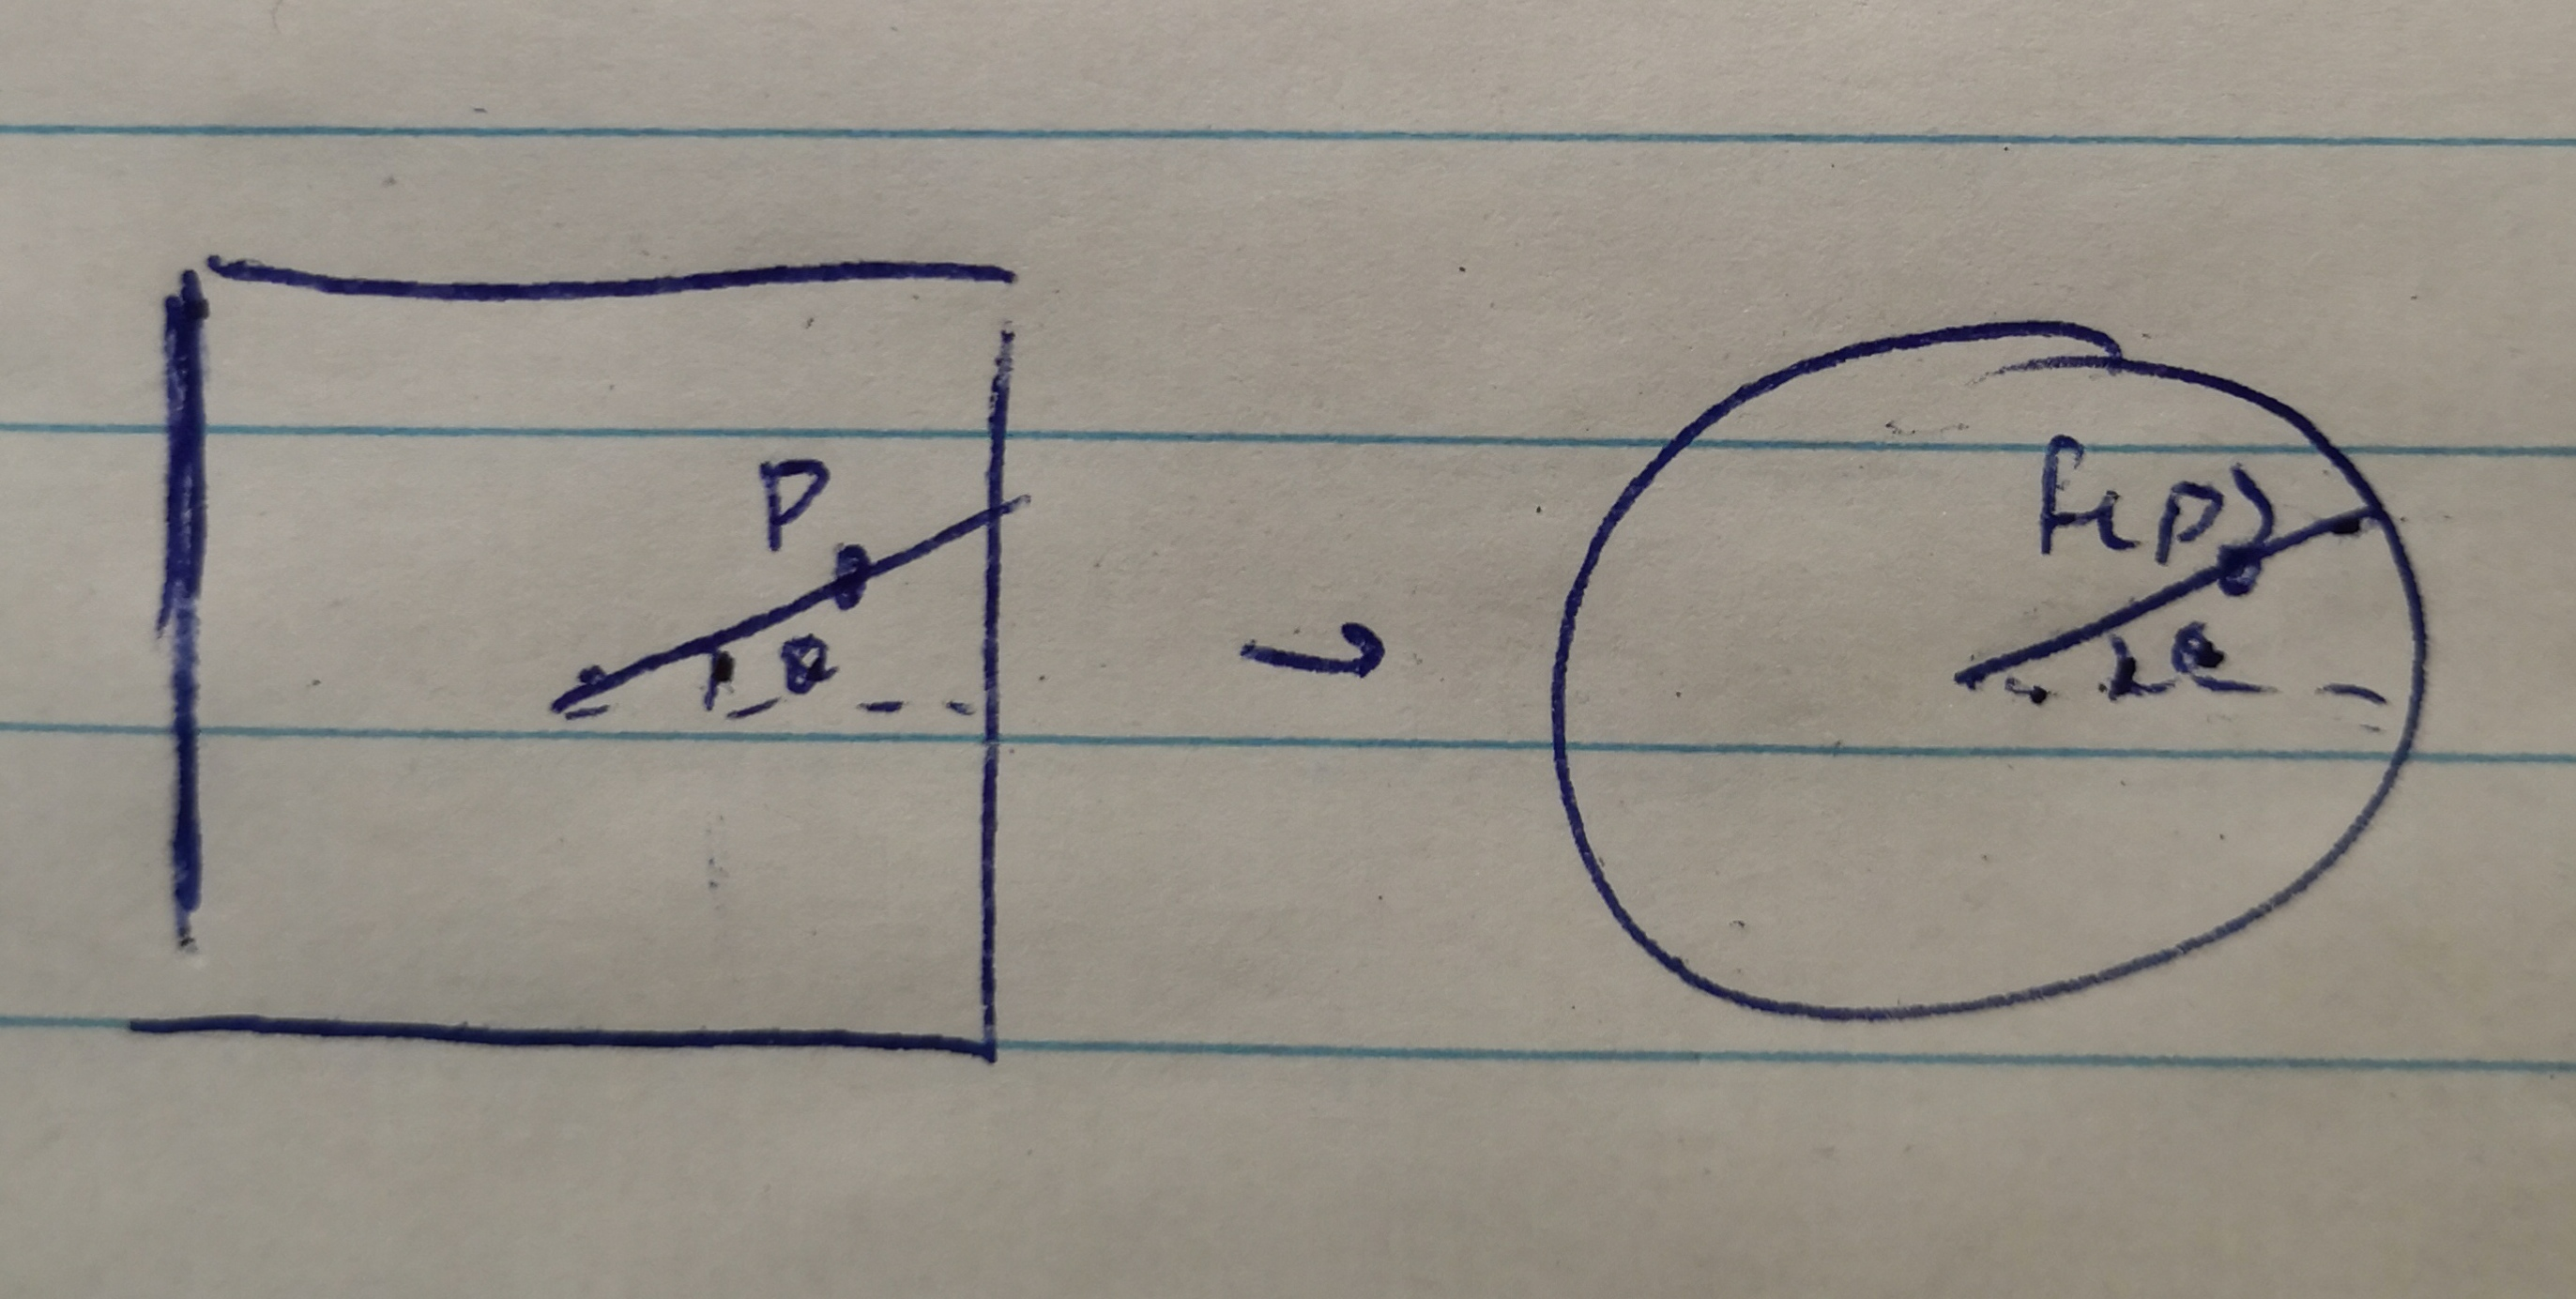
\includegraphics[width=0.9\linewidth]{fig1.jpg} 
\label{fig:wrapfig}
\end{wrapfigure}

We construct a function that "stretches" $I$ into $D$. That is, we take the center of $I$ to be $o = (1/2,1/2)$ and for each point in $I$, map it to a point in $D$, preserving polar angle and the ratio of distance to the center. In particular, let $d(p,o) = d$ and the ray from $o$ through $p$ intersect the edge of $I$ at $q$, $d(q,o) = R$. Also let the signed angle of the ray to the horizontal be $\theta$. we map $p$ to a point $\frac{d}{R}\frac{1}{R}$ away from the center of $D$ with signed angle $\theta$ to the horizontal. This function can be modeled as:
$$f(1/2,1/2) = (0,0)$$
$$f(x,y) = \left((x-1/2)\cdot r(x,y), (y-1/2)\cdot r(x,y) \right) \text{ otherwise,}$$
$$\text{where } r(x,y) = \frac{4\cdot\sqrt{(x-1/2)^2+(y-1/2)^2}}{1 + \left(\frac{\min(|x-1/2|,|y-1/2|)}{\max(|x-1/2|,|y-1/2|}\right)^2}$$
\begin{figure}[h!]
\centering
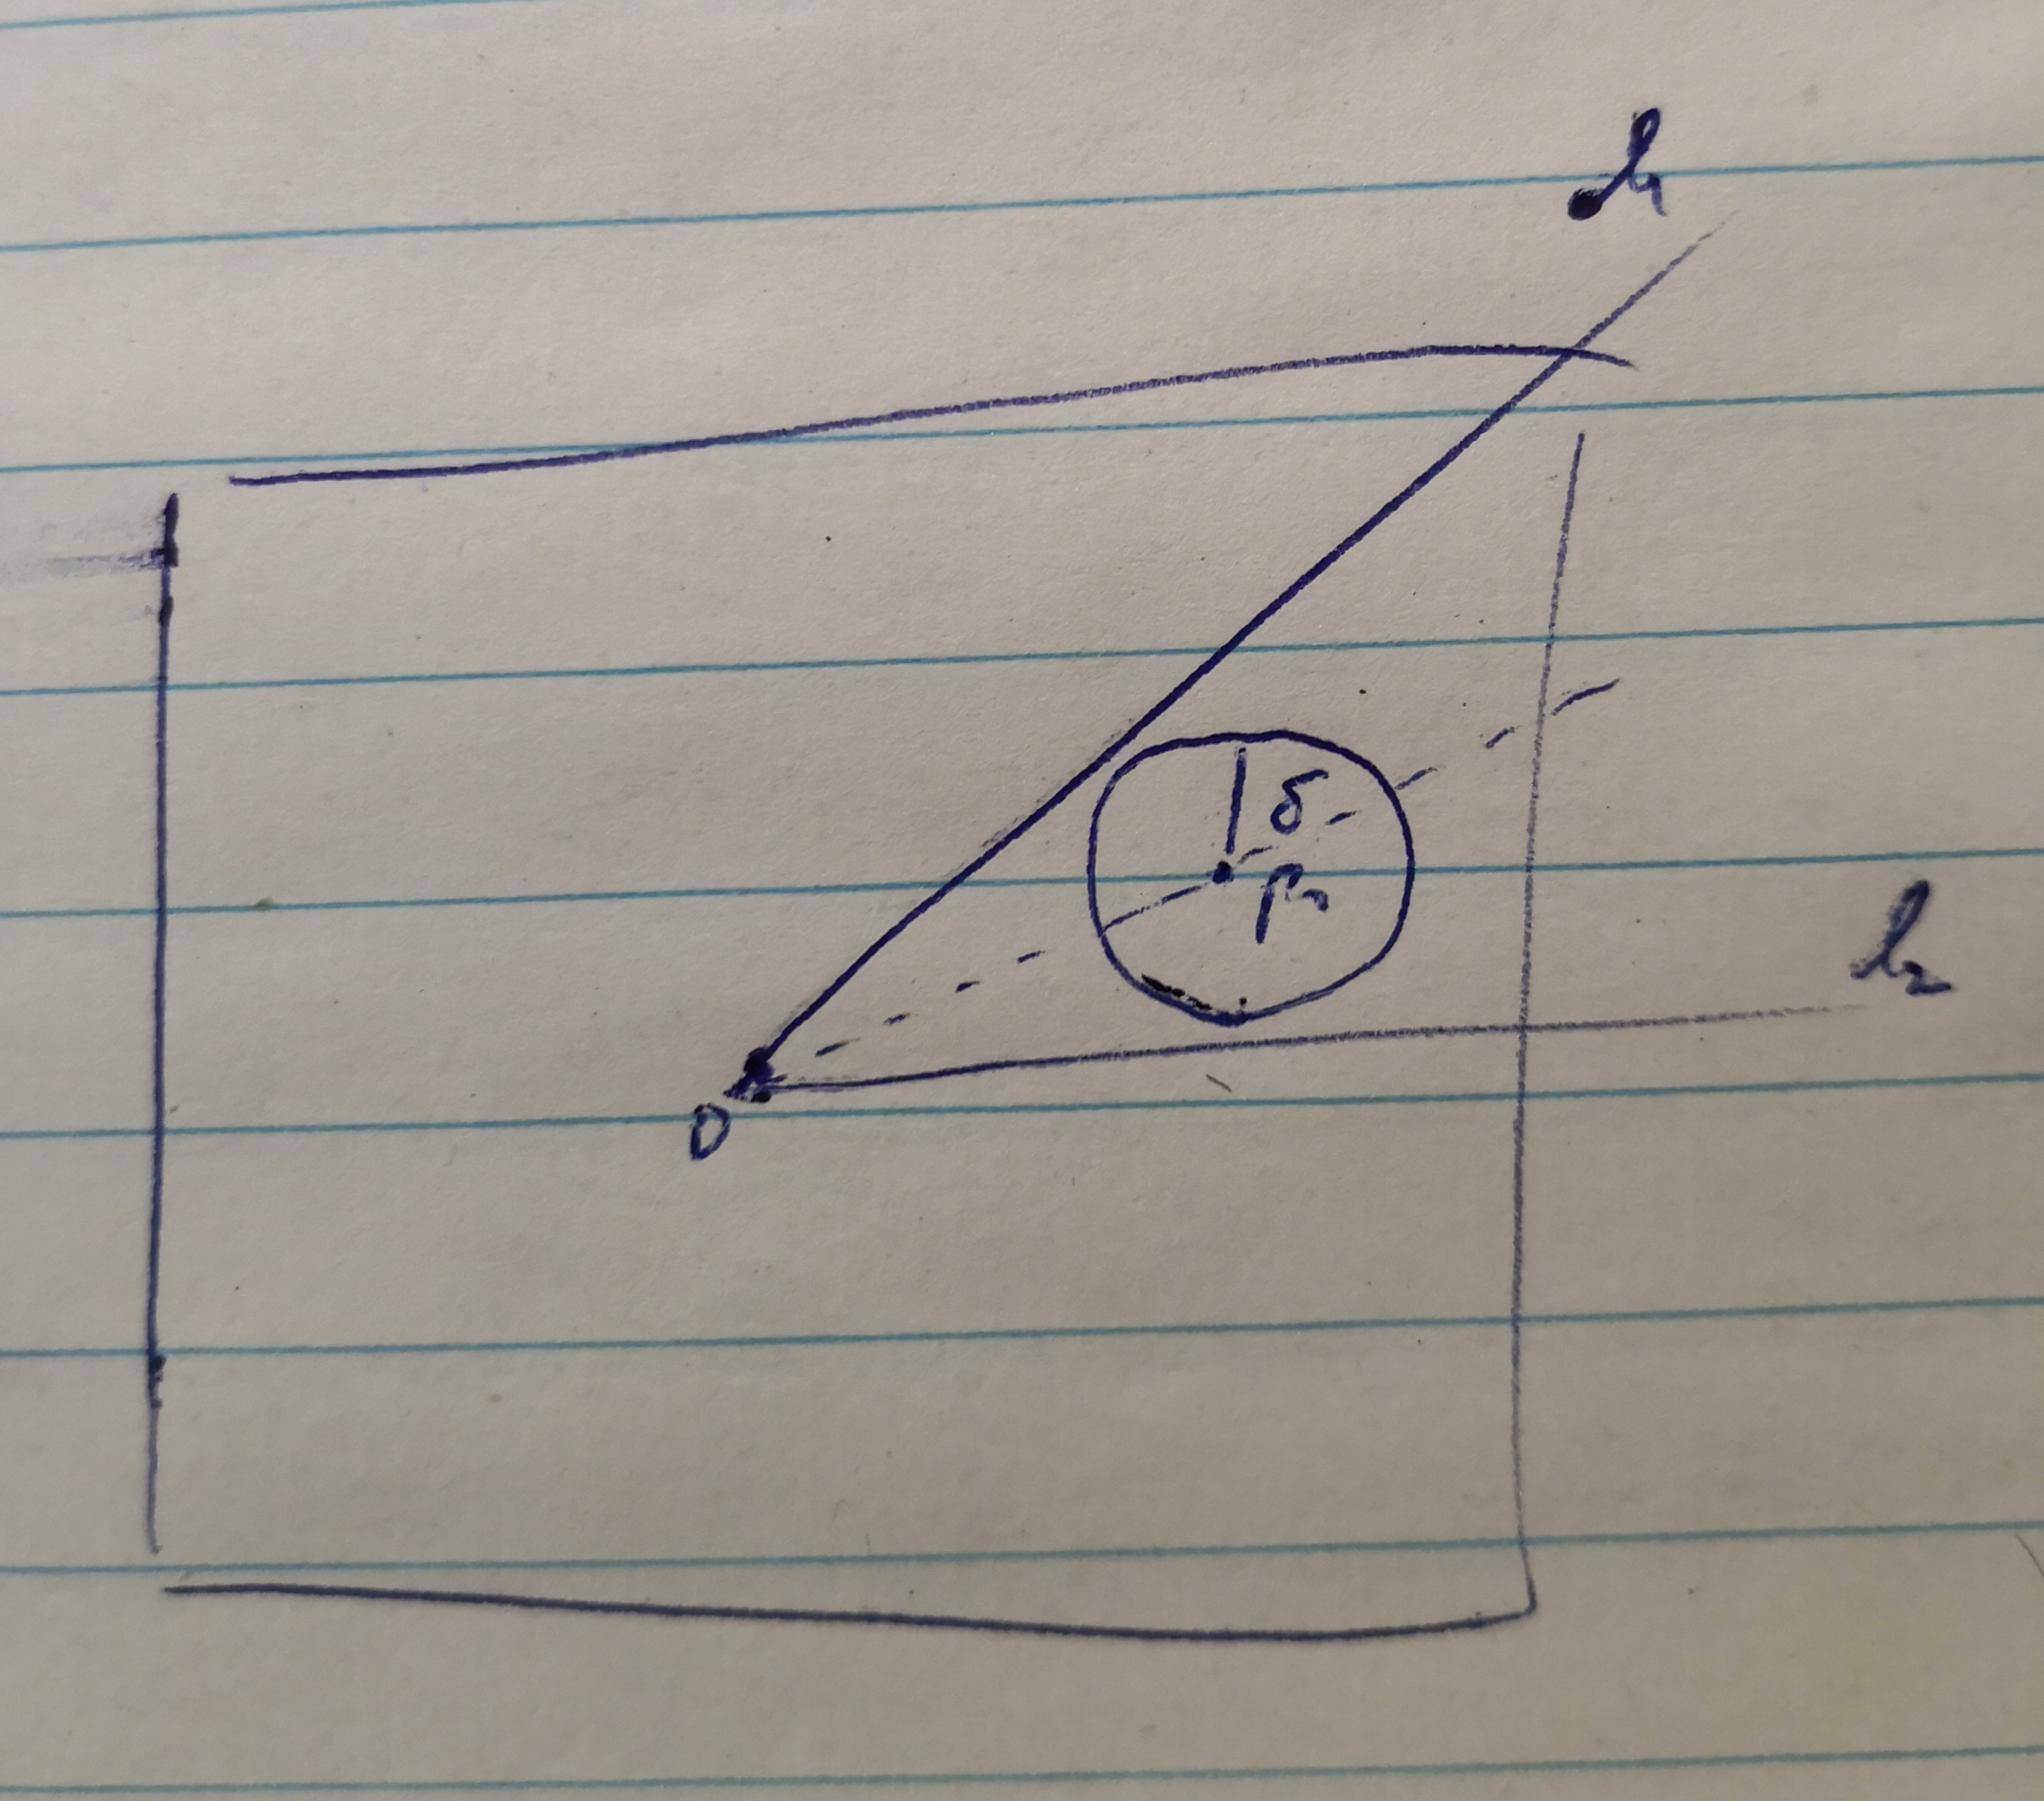
\includegraphics[scale=0.06]{fig2.jpg}
\label{fig:universe}
\end{figure}


This is somewhat nasty to look at directly, but note to prove continuity of $f$ it suffices to prove it at $(1/2,1/2)$ and show that $\frac{\min(|x-1/2|,|y-1/2|)}{\max(|x-1/2|,|y-1/2|}$ is continuous away from $(1/2,1/2)$.\\
For simplicity denote this function $g(p) = \frac{\min(|x-1/2|,|y-1/2|)}{\max(|x-1/2|,|y-1/2|}$ where $p = (x,y)$. Note that $g$ represents the minimum of the slope or the inverse of the slope of the line through $o$ and $p$. WLOG fix $p_0$ in $I$ with corresponding slope $g = \alpha$ s.t. $\alpha < 1$. (If $\alpha > 1$, the analysis can be done similarly by swapping the roles of the $x$ and $y$ axes.) For any $\epsilon > 0$ we can draw lines $\ell_1$ with slope $\alpha + \epsilon$ and $\ell_2$ with slope $\alpha - \epsilon$, through $o$. Since $I$ is compact, we can always find $\delta $ less than both the distances from $p_0$ to $\ell_1$ and $\ell_2$. And thus neither line intersects the ball of radius $\delta$ around $p_0$. Hence, for $p$ s.t. $d(p,p_0) < \delta$, $g(p)$ is between $\alpha + \epsilon$ and $\alpha - \epsilon$, that is $d(g(p),g(p_0)) < \epsilon$.\\
Now prove continuity at $(1/2,1/2)$:\\
By construction, if $d(p,o) < \delta$, then $d(f(p),f(o)) < 4\delta$, since $R \geq 1/2$, so $\frac{d}{R}\frac{1}{R} \leq 4d < 4\delta$. So for $\epsilon > 0$ we can pick $\delta = \epsilon / 4$ to prove continuity.\\
By construction, this function is one-to-one:\\
For points $p\neq q$ away from $(1/2,1/2)$, either the angle $\theta$ or length ratio $\frac{d}{R}$ is different, so they will be either be sent to points on different rays or different points on the same ray. In either case, they'll be sent to different points away from $(0,0)$, which is the image of $(1/2,1/2)$.\\
This function is also onto:\\
Note that in $I$ we can find a point with any angle $0\leq\theta<2\pi$ and length ratio $0<\frac{d}{R}\leq 1$, so any point in $D$ away from $(0,0)$ can be expressed in polar as $(\theta,r)$, $0\leq\theta<2\pi, 0<r\leq1$, and thus has a pre-image in $I$ away from $(1,2,1,2)$, which is the pre-image for $(0,0)$. $\Box$

\section{}
\subsection{}
Consider sequence $(x_k) = (f^k(q))$ for arbitrary $q \in X$. This is a Cauchy sequence:\\
By contraction property, for any $k$, $d(x_{k+1},x_{k+2}) = d(f(x_{k}),f(x_{k+1})) \leq \alpha \cdot d(x_k,x_{k+1})$. So by induction, $d(x_k,x_{k+1}) \leq \alpha^k \cdot d(x_0,x_1)$. Now note for $n<m$, by Triangle inequality,
\begin{equation*}
    \begin{split}
        d(x_n,x_m) &\leq d(x_n,x_{n+1}) + d(x_{n+1},x_{n+2}) + \dots + d(x_{m-1},x_m)\\
        &= d(x_n,x_{n+1})[1 + \alpha + \alpha^2 + \dots + \alpha^{m-n-1}]\\
        &= d(x_n,x_{n+1}) \frac{1-\alpha^{m-n}}{1-\alpha} < d(x_n,x_{n+1}) \frac{1}{1-\alpha}\\
        &\leq \frac{\alpha^n}{1-\alpha} d(x_0,x_1)
    \end{split}
\end{equation*}
Note that $1 - \alpha$ and $d(x_0,x_1)$ are constants, so for every $\frac{\epsilon (1-\alpha)}{d(x_0,x_1)} > 0$ we can find $N$ s.t. $\alpha^N < \frac{\epsilon (1-\alpha)}{d(x_0,x_1)}$, so that $d(x_n,x_m) \leq \frac{\alpha^N}{1-\alpha} d(x_0,x_1) < \epsilon$ for $n,m \geq N$. So the sequence is Cauchy.\\
$X$ is compact, so $(x_k)$ converges to some $p \in X$. In addition, as shown in class, contractions are uniformly continuous, so $f$ is continuous. So by definition of continuity,
$$\lim\limits_{k\rightarrow\infty} x_k = p$$
$$\lim\limits_{k\rightarrow\infty} f(x_k) = f(p)$$
$$\lim\limits_{k\rightarrow\infty} x_{k+1} = p = f(p)$$
Now that have proved existence, we prove uniqueness:\\
Suppose there are fixed points $p,q$ s.t. $p\neq q$. Then $f(p) =p$ and $f(q)=q$. But now $d(f(p),f(q) = d(p,q) \nless \alpha \cdot d(p,q)$ $\contra$

\subsection{}
Note $d(f^{k+1}(q),f(p)) \leq \alpha\cdot d(f^k(q),p)$ for all $q \in X$. Since $f(p) = p$, $d(f^{k+1}(q),p) \leq \alpha\cdot d(f^k(q),p)$, which implies $f^k(q) \rightarrow p$ for all $q$ $\Box$

\subsection{}
First prove the sequence $(x_k) = (g^k (q)$ is Cauchy for arbitrary $q \in X$:\\
Consider subsequences $(x_{mk}),(x_{mk+1}),\dots (x_{mk+m-1})$ and denote them\\
$(y_0),(y_1), \dots (y_{m-1})$. Note that every $x_k$ is in some sequence $(y_i)$. Each of these subsequences can be written as $(g^i (q) \cdot g^{mk}(q)) = (g^i (q) \cdot f^{k}(q))$ so is Cauchy and converges to $p$. Now for every $\epsilon / 3$ we can find $N_i$ for each $(y_i)$ s.t. $d(y_{i,n},p) \leq \epsilon /3$ for $n\geq N_i$. Since there are finitely many such $N_i$, we may take $N$ to be the maximum of these $N_i$. Then for $n,l \geq m(N+1)$, by Triangle $d(x_n,x_l) \leq d(x_n,p) + d(p,x_l) \leq \epsilon/3 + \epsilon/3 < \epsilon$.\\
Since $(x_k)$ is Cauchy and a subsequence converges to $p$, $x_k = g^k (q)\rightarrow p$. Note that we chose $q$ arbitrary, so all $g^k (q) \rightarrow p$, proving (b). Then by the logic in (a), this suffices to show existence and uniqueness of fixed point $p$, proving (a) $\Box$

\section{}
\subsection{}
Since there are finitely many terms in $A$, put $a = \max\limits_{i,j} \{a_{i,j}\}$. Take $\epsilon > 0$ and fix some vector $x$. Consider $y$ s.t. $d(x,y) < \frac{\epsilon}{an}$. For all $i$,
\begin{equation*}
    \begin{split}
        |(Ax)_i - (Ay)_i| &= |\sum\limits_{j}a_{i,j}x_j - \sum\limits_{j}a_{i,j}y_j|\\
        &= |\sum\limits_{j}a_{i,j}(x_j-y_j)|\\
        &\leq \sum\limits_{j} a_{i,j} |x_j - y_j|\\
        &< an\cdot \frac{\epsilon}{an} = \epsilon
    \end{split}
\end{equation*}
So $d(f(x),f(y))<\epsilon$ and $f$ is continuous $\Box$

\subsection{}
Note $X$ is closed and bounded in $\mathbb{R}^n$ so is compact. Since all $a_{i,j} > 0$ and the matrix is finite, we can find $\gamma > 0$ s.t. all $a_{i,j} > \gamma$. Now we can take $\gamma\geq\beta > 0$ s.t. $n\beta < 1$. Now let $b_{i,j} = \frac{a_{i,j}-\beta}{1-n\beta} > 0$. Note that the matrix $B$ of such $b_{i,j}$ is also a stochastic matrix, since $\sum\limits_{j}b_{i,j} = \frac{\sum\limits_{j}(a_{i,j} - \beta)}{1-n\beta} = \frac{1-n\beta}{1-n\beta} = 1$ and similarly for columns. Now note that for vectors $x,y$ and all $i$,
\begin{equation*}
    \begin{split}
        |(Bx)_i - (By)_i| &= |\sum\limits_{j}b_{i,j}x_j - \sum\limits_{j}b_{i,j}y_j|\\
        &= |\sum\limits_{j}b_{i,j}(x_j-y_j)|\\
        &\leq \sum\limits_{j} b_{i,j} |x_j - y_j|\\
        &\leq \sum\limits_{j} b_{i,j} d(x,y)\\
        &= d(x,y)
    \end{split}
\end{equation*}
and
\begin{equation*}
    \begin{split}
        |(Ax)_i - (Ay)_i| &= |\sum\limits_{j}a_{i,j}x_j - \sum\limits_{j}a_{i,j}y_j|\\
        &= |\sum\limits_{j}a_{i,j}(x_j-y_j)|\\
        &= |\sum\limits_{j}(b_{i,j}(1-n\beta) + \beta)(x_j-y_j)|\\
        &= |\sum\limits_{j} b_{i,j}(1-n\beta)(x_j - y_j) + \beta\sum\limits_{j} x_j - \beta\sum\limits_{j} y_j|\\
        &= |\sum\limits_{j} b_{i,j}(1-n\beta)(x_j - y_j)|\\
        &= (1-n\beta)|\sum\limits_{j}b_{i,j}(x_j-y_j)|\\
        &\leq (1-n\beta) d(x,y)
    \end{split}
\end{equation*}
so $f$ is a contraction with $\alpha = 1-n\beta$, as desired $\Box$

\subsection{}
Note that this sequence is a Markov Chain with state space $S = \{0,1,2\}$ and transition matrix $P = \begin{bmatrix}
  1/2 & 1/4 & 1/4\\ 
  1/4 & 1/2 & 1/4\\
  1/4 & 1/4 & 1/2
\end{bmatrix} $. By inspection, $P$ satisfies the conditions specified in (b), so is a contraction on $X$, the space of suitable probability distribution vectors. Note that $X$ is compact, so there exists unique stationary probability distribution $\pi$ s.t. $x \rightarrow \pi$ for all $x \in X$. Clearly, $\pi = (1/3,1/3,1/3)$ is a solution to $Pv = v$, so all $x\rightarrow \pi$ In other words, Prob$(x_n=0) \rightarrow 1/3$, Prob$(x_n=1) \rightarrow 1/3$, Prob$(x_n=2) \rightarrow 1/3$, as desired $\Box$

\subsection{}
We may label the icosahedron's vertices from 1-12 and assign weight of $1/5$ to all edges. The ant's walk can be modeled as a Markov chain with states $\{1,2,\dots12\}$ and transition matrix $P$ defined as $P_{i,j} = 1/5$ if there is an edge between vertex $i$ and $j$, and $P_{i,j} = 0$ otherwise.
We may verify this is a valid stochastic matrix by observing the $i$-th row and column corresponds to the sum of weights of edges from the $i$-th vertex, which is 1 by construction. We need to do a little more work to fit all the conditions in (b):\\
Note that the Markov chain is aperiodic, since by construction, all states are strongly connected and $P^2_{0,0} = 1/5 > 0$. So there must exist some $m$ s.t. any state $i$ can reach any other state $j$ in m steps. Thus, $P^m$ contains no zero entries and is thus a contraction on the (compact) space of probability distributions $X$. Thus, $P^m$ has unique $\pi$, and by 2(c) it is also the unique $\pi$ for $P$. We can easily verify $\pi = (1/12,1/12,\dots 1/12)$.\\
The probability that the ant ends at state $i$ in $n$ steps, given it starts at state $i$ is simply $p_n = (P^n\alpha)_i$, where $\alpha$ is the initial probability distribution, with $\alpha_j = 1$ if $j=i$ and $\alpha_j = 0$ otherwise. $P^n\alpha \rightarrow \pi$, so $p_n \rightarrow \pi_i = 1/12$ $\Box$

\end{document}
